\documentclass[8pt]{beamer}
%epackage[french]{babel}
\usepackage[latin1]{inputenc}
\usepackage{listings}
\usepackage{times}
\usepackage{wasysym}
\usepackage[T1]{fontenc}

\usepackage{listings}

\definecolor{mongris}{gray}{0.8}           % definition couleur grise
\newcommand{\dd}{\footnotesize $\Diamond$}

\newcommand{\HH}{ \vspace{0.5pt}\hrule}
\newcommand{\round}[1]{\lceil #1 \rfloor}  % notation arrondi
\def\eme{$^{\textrm{{\`e}me}}$}                  % i {\`e}me
\def\num{n^{\circ}}                        % numero
\def\Num{N^{\circ}}                        % Numero
\def\sinc{\mathrm{sinc}}                   % sinus cardinal
\def\ere{$^{\textrm{{\`e}re}}$}                % {\`e}re
\def\er{$^{\textrm{{e}r}}$}                % {\`e}re
\def\eg{\emph{e.g.} }                      % e.g.
\def\ie{\emph{i.e.} }                      % i.e.
\def\etc{\emph{etc}}                       % etc
\def\cm{\,cm}                              % cm
\def\met{\,m}                              % m
\def\mm{\,mm}                              % mm
\def\deg{$^\circ$}                         % degres
\def\ud{\mathrm{d}}                        % pour dx dy ...


\def \R {{\Bbb R}}
\def \I {{\Bbb I}}
\def \H{{\Bbb H}}
\def \F {{\Bbb F}}
\def \S {{\Bbb S}}
\def \B {{\Bbb B}}
\def \Z {{\mathbb Z}}
\def \G {{\mathbb G}}
\def \L {{\mathcal{L}}}
\def \C {{\mathcal C}}
\def \P {{\mathcal P}}
\def \Q {{\mathcal Q}} 
\def \E{{\mathcal E}}
\def \D{{\mathcal D}}
\definecolor{mybluecolor}{RGB}{116,121,149}

\newcommand{\darky}[1]{{\usebeamercolor[fg]{block title example} #1}}
\newcommand{\myblue}[1]{{\color{mybluecolor}\aut{[#1]}}}

\newcommand{\ball}  {\ensuremath{B}}
\newcommand{\AMDR}{\operatorname{AMD}}
\newcommand{\AMD}{\operatorname{AMD}}

\newcommand{\MAset}{\ensuremath{\mathrm{A\!M}} }
\newcommand{\MAsetg}{\ensuremath{\MAset^g } }

\def \PS {{\aut{Planar-4-3-SAT}}}
\def \R {{\Bbb R}}
\def \I {{\Bbb I}}
\def \F {{\Bbb F}}
\def \S {{\Bbb S}}
\def \Z {{\mathbb Z}}
\def \L {{\mathcal{L}}}
\def \C {{\mathcal C}}
\def \P {{\mathcal P}}
\def \Q {{\mathcal Q}} 
\def \E{{\mathcal E}}
\def \D{{\mathcal D}}
\def \BD {{\bar{\mathcal{D}}}}
\def \etal {{\it et al.~}}
\def\arc{\mbox{arc}}
\definecolor{mongris}{gray}{0.8}          
\newcommand{\fup}[1]{\uparrow#1\uparrow}
\newcommand{\fdown}[1]{\downarrow#1\downarrow}
\newcommand{\sI}[1]{\overline{\tt #1}}
\newcommand{\iI}[1]{\underline{\tt #1}}
\newcommand{\e}[5]{#1 & #2 & #3 & #4 & #5 \\}
\newcommand{\eh}[5]{\text{#1} & \text{#2} &  \text{#3} &  \text{#4} & \text{#5}\\} 

\usepackage{beamerthemeliris2}
\useoutertheme{smoothbars}

\title[GT G�om�trie Discr�te]{DGtal}
\subtitle{\url{http://liris.cnrs.fr/dgtal}}

%\author{D. Coeurjolly}
\author{David Coeurjolly}


 \newcommand{\fod}[2]{\multicolumn{2}{p{3.5cm}}{\emph{#1}\dotfill} &
      \multicolumn{2}{p{9cm}}{#2}\\}
    \newcommand{\fodt}[4]{\emph{#1} & {\footnotesize \textsl{#2}} & #3 & \small #4\\}
    % \newenvironment{ta}{\begin{tabular}{p{3.5cm}p{9cm}}}{\end{tabular}\\}
    \newenvironment{ta}{\begin{tabular}{crll}}{\end{tabular}\\}
    % \vfill


\newcommand{\aut}[1]{{\sc #1}}             % auteur en small capsu


%\institute%[XXX]
%{%
%
%  {\bf Laboratoire d'InfoRmatique en Image et Systèmes d'information} \\
%  { \scriptsize{
%  LIRIS UMR 5205 CNRS/INSA de Lyon/Université Claude Bernard Lyon 1/Université Lumiè%re Lyon 2/Ecole Centrale de Lyon\\
%  INSA de Lyon, bâtiment J. Verne\\
%  20, Avenue Albert Einstein - 69622 Villeurbanne cedex\\
%  \url{http://liris.cnrs.fr}}
%  }
%}



\graphicspath{{./Figures/}, {./../images/},{./Fig/}, {./ICPR2010/},{./Antoine/images/}; {./Images/}}


\begin{document}

\small






\begin{frame}[plain]
  \titlepage
\end{frame}

%------------------------------------------------------------------------------
\begin{frame}%[allowframebreaks]
  \frametitle{DGtal: why, who}
  
  \small
  \begin{block}{Objectives}
    \small
    \begin{itemize}
    \item to make digital geometry easier for the neophyte (student,
      researcher from another field, \ldots)
    \item to quickly test  new ideas, with objective comparison wrt
      existing works
    \item to make easier the implementation of demonstrators
    \item to help spread our research results to other domains
    \end{itemize}
  \end{block}
  
\alert{$\Rightarrow$ Federative Project}
  
  \small
  \begin{block}{Who ? (for now) \ldots}
    \small
    \begin{columns}
      \begin{column}{0.45\textwidth}
        \begin{itemize}
        \item LIRIS (Lyon)      
        \item Gipsa-lab (Grenoble)
        \item GREYC (Caen)
        \end{itemize}
      \end{column}
      \begin{column}{0.45\textwidth}
        \begin{itemize}
        \item LAMA (Chamb�ry)
        \item LORIA (Nancy)
        \item IRCCyn (Nantes)
        \end{itemize}
      \end{column}
    \end{columns}
  \end{block}
\end{frame}
%------------------------------------------------------------------------------
%------------------------------------------------------------------------------
\begin{frame}%[allowframebreaks]
  \frametitle{DGtal: what for ?}
  
  \small
  \begin{block}{Main features}
    \small
    \begin{itemize}
    \item to define digital objects in arbitrary dimension
    \item to propose algorithms for topological and geometric analysis
    \item to provide I/O mechanisms and visualization tools
    \end{itemize}
  \end{block}
  \medskip

 \hspace*{-1cm} \begin{tabular}{cccccc}
    \includegraphics[height=0.07\textheight]{exampleDSS-3}
    &
    \includegraphics[height=0.07\textheight]{geomDCA}
    &
    \includegraphics[height=0.1\textheight]{edt-2d}
    &
    \includegraphics[height=0.1\textheight]{object-3d-18-6}
    &
    \includegraphics[height=0.1\textwidth]{thinning-3d}
    &
    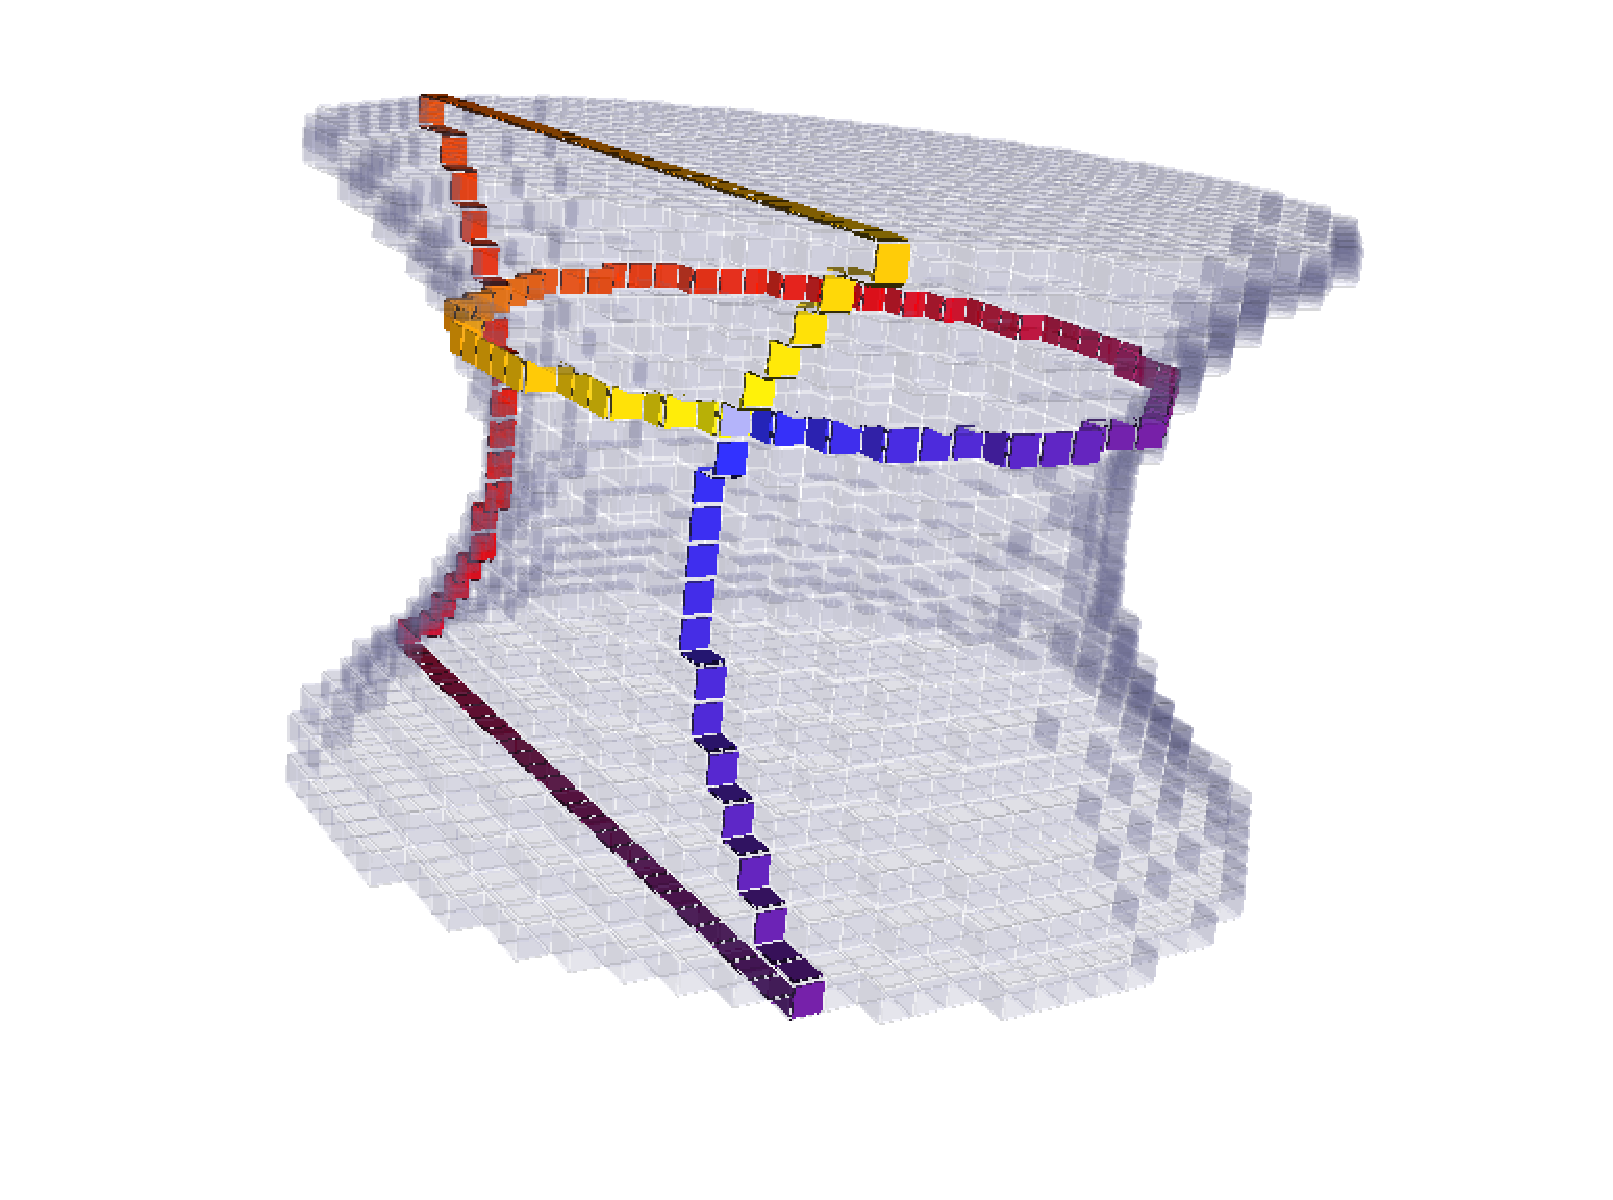
\includegraphics[height=0.1\textwidth]{surfelTracking}
    \\
    DSS & DCA & DT & Objects & Thinning & Cellular model\\
    \includegraphics[height=0.15\textheight]{lengths-ball-R10-bis}
    &
    \includegraphics[height=0.15\textheight]{normal}
    &
    \includegraphics[height=0.1\textheight]{shapes}
    &
    \includegraphics[height=0.1\textheight]{mpolynomial}
    &
    \includegraphics[height=0.1\textwidth]{klokanNoise}
    &
    \ldots
    %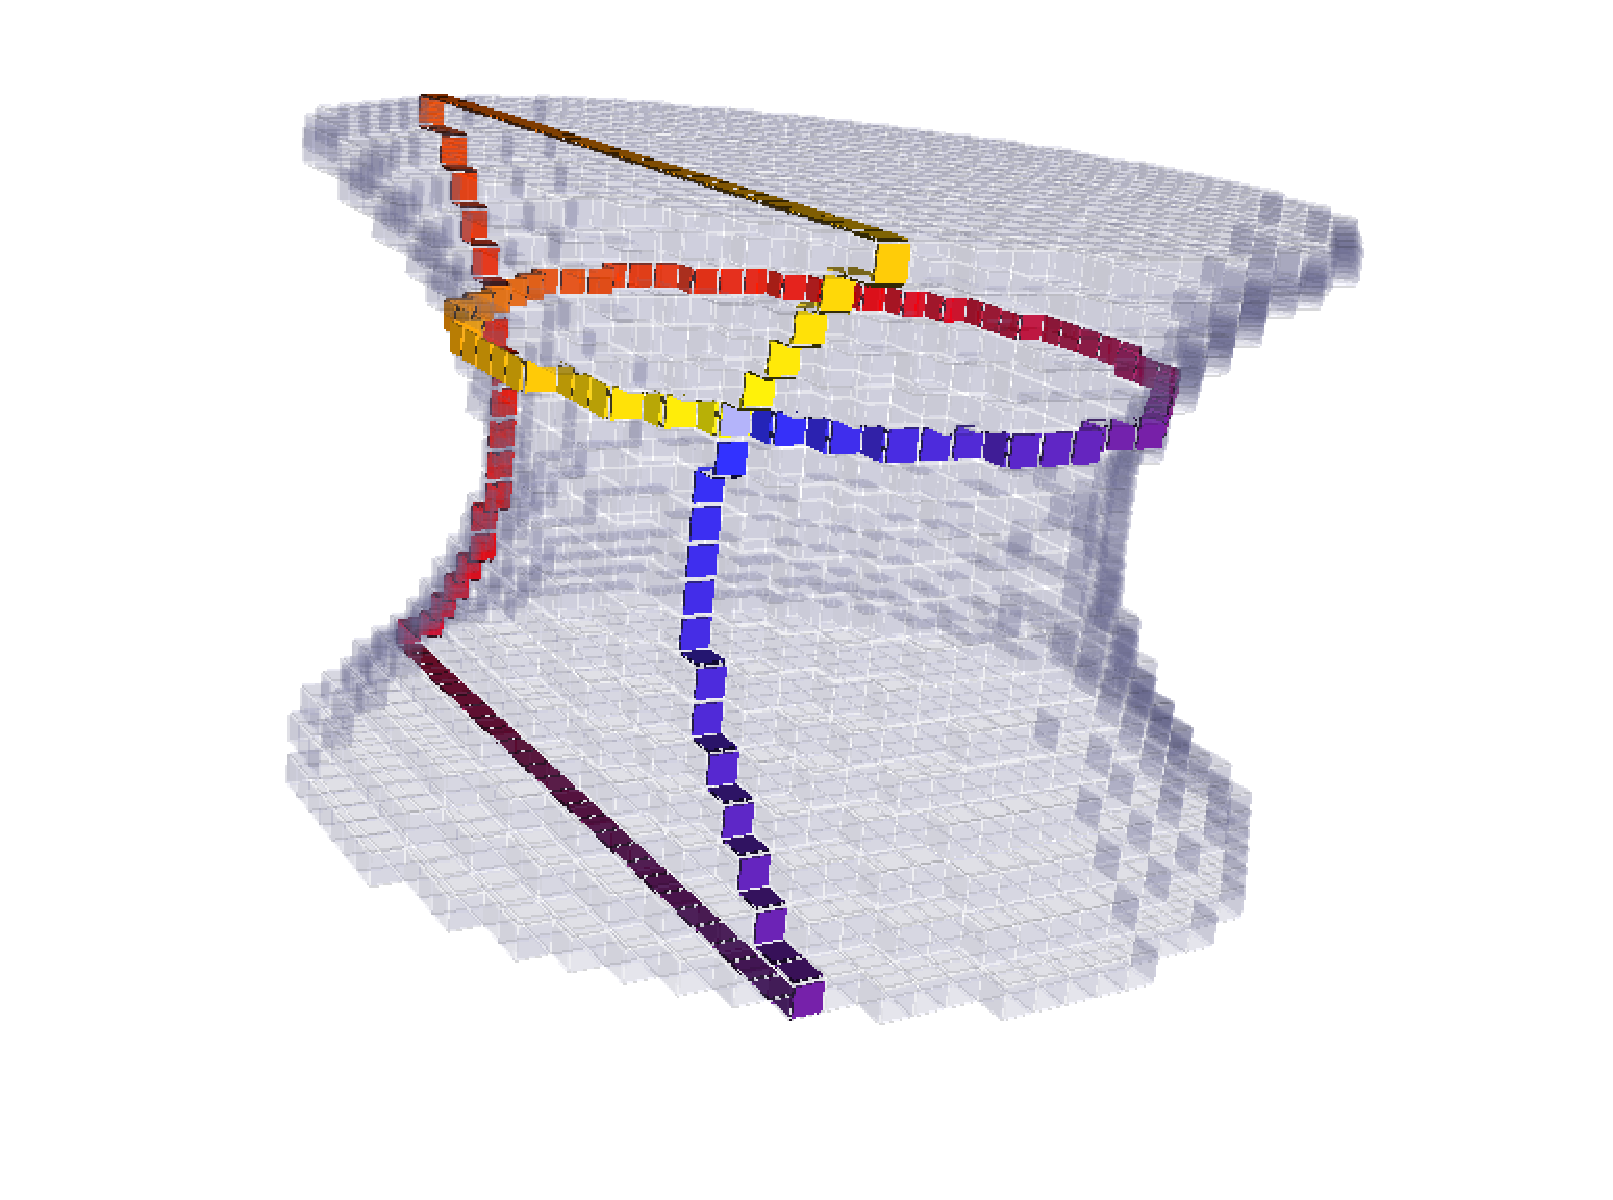
\includegraphics[height=0.15\textwidth]{surfelTracking}
    \\
    Estimators & normal vectors & Shape DB & polynomial surfaces& Contours & 
 \end{tabular}
 
\end{frame}
%------------------------------------------------------------------------------
%------------------------------------------------------------------------------
\begin{frame}%[allowframebreaks]
  \frametitle{DGtal philosophy and structure}

  \begin{block}{}
    \small
    \begin{itemize}
    \item  Genericity and efficiency: C++ library, concepts
    \item  LGPL
    \item Cmake build system (linux/macOS/MSwindows)
    \item user friendly, not necessarily kernel-developer friendly
    \end{itemize}
  \end{block} 
  \begin{alertblock}{\centering Kernel Package\HH}
            \small
          \begin{itemize}
          \item Digital space
          \item  Point, vectors
            \item Digital domains and digital sets
             \item  \ldots  
          \end{itemize}
       
   \end{alertblock}

 \begin{alertblock}{\centering Arithmetic Package\HH}
    \footnotesize
    \begin{itemize}
  \item  Fractions
  \item Irreducible fractions 
\item DSS Pattern..
    \item \ldots
    \end{itemize}
  \end{alertblock}

  
\end{frame}




\begin{frame}
  \frametitle{DGtal philosophy and structure}
  \begin{alertblock}{\centering Topology Package\HH}
    \small
       \begin{itemize}
    \item Digital Topology: connectedness, border, simple points
      (\emph{a la} Rosenfeld)
    \item Cartesian Cellular Topology: cells,  surfaces and contours
      (\emph{a la} Herman), tracking algorithms
    \item Digital Surface concepts and models
    \end{itemize}
  \end{alertblock}
    \begin{alertblock}{\centering Geometry Package\HH}
    \small
    \begin{itemize}
    \item Primitives (\emph{a.k.a.} \textsc{SegmentComputers}): DSS, DCA,...
    \item Contour analysis: decomposition, convexity, estimators
    \item Volumetric analysis: area/volume, distance transforms,
      reverse distance transforms, Fast-marching methods.
    \item Implicit/parametric shape generator for multigrid analysis
    \end{itemize}
  \end{alertblock}
\begin{alertblock}{\centering Math Package\HH}
    \footnotesize
    \begin{itemize}
    \item Representation of polynoms
    \item \ldots
    \end{itemize}
  \end{alertblock}
\end{frame}

\begin{frame}
  \frametitle{DGtal philosophy and structure}

  \begin{alertblock}{\centering Image Package\HH}
    Image concept and Image containers, e.g.
    \begin{itemize}
    \item Image by STL \texttt{vector} (linearized nD image)
    \item Image by STL \texttt{map} (mapping points$\leftrightarrow$values)
    \item HashTree image container (generalized octree with hashing functions)
    \end{itemize}
  \end{alertblock}
  

  \begin{alertblock}{\centering IO Package\HH}
    \small
    \begin{itemize}
    \item \texttt{Boards}: export to illustrate objects/algorithms (eps,pdf,svg,png,tikz\ldots)  
    \item \texttt{Viewers}:  simple 3D viewer (Qt/QGlViewer)
    \item Readers/writers for various image formats
    \end{itemize}
  \end{alertblock}
\end{frame}
%------------------------------------------------------------------------------
%------------------------------------------------------------------------------
\begin{frame}%[allowframebreaks]
  \frametitle{DGtal 0.5.1}

\begin{itemize}
\item Project started in Jan 2010
\item 200k lines of code
\item $env.$ 557 C++ classes 
\item Used in couple of research projects (ANR digitalSnow,
  collaboration with Chemical lab in Lyon, collaboration with
  Agricultural in Nancy,... )
\end{itemize}
  
\end{frame}

\begin{frame}
  \frametitle{DGtal Projects}

  \begin{block}{DGtal\HH}
    Main library (classes + unit tests + example programs + documentation files)
  \end{block}

\vspace{0.5cm}

  \begin{block}{DGtalTools\HH}
   Command line tools built using DGtal (multigrid shape generators,
   contour analyzers, file format conversion,...)
  \end{block}

\vspace{0.5cm}

  \begin{block}{DGtalScripts\HH}
    Scripts and template files to generate new classes/unit tests files
  \end{block}
\end{frame}




\begin{frame}
  \includegraphics[width=12cm]{IMG_0581}
\end{frame}

\begin{frame}
  \frametitle{Roadmap/Wishes}

  \begin{itemize}
  \item Linear Algebra Package: exact sign to determinant, ...
  \item Enhance bindings with other libs through image containers:
    Olena, VIGRA...
    \item More geometric primitives 
    \item Affine transformations
    \item Path based Distance Transformation (+ MA, + ReverseDT...)
    \item  Digital Partition models
    \item Polytope representation in $\mathbb{R}^n/\mathbb{Z}^n$
  \end{itemize}
\end{frame}



\begin{frame}
  \frametitle{Interact with DGtal}

  \begin{block}{Feedbacks\HH}
    \begin{itemize}
    \item Test the build
    \item Report issues
    \item Review the doc
    \end{itemize}
  \end{block}

  \begin{block}{Goals\HH}
    Help us ``prioritizing'' the Todos/ new features
  \end{block}

  \begin{block}{Get involved\HH}
    \begin{itemize}
    \item  Development of new DGtalTools
    \item Development of  new DGtal features
    \item \ldots
    \end{itemize}
  \end{block}


\end{frame}

\end{document}


%Sample.dat -> GRidCurve -> board (GC, GC::Arrows, GC::Inci)

%Image -> Set ->  DT -> board

%Image -> contour (KSpace, track) -> GC -> estimateur (longueur)

%Shape -> Digitizer -> Contour -> GC -> Estimateur

% Shape -> surface -> viewer

% Shape -> Surface -> slice -> GC -> longueur (viewer Segm.DSS)
